%
% introduction.tex
%
% Copyright (C) 2022 by Universidade Federal de Santa Catarina.
%
% GNSS Networks Based on Small Satellites
%
% This work is licensed under the Creative Commons Attribution-ShareAlike 4.0
% International License. To view a copy of this license,
% visit http://creativecommons.org/licenses/by-sa/4.0/.
%

%
% \brief Introduction chapter.
%
% \author Gabriel Mariano Marcelino <gabriel.mm8@gmail.com>
%
% \version 0.0.0
%
% \date 2019/11/30
%

\chapter{Introduction} \label{ch:introduction}

This work proposes the study, feasibility verification, and implementation of a network of a Global Navigation Satellite System (GNSS\nomenclature{\textbf{GNSS}}{Global Navigation Satellite System.}) based on small satellites, especially nanosatellites, or specifically CubeSats.

The use of small satellites has been growing exponentially in recent years, as can be seen in \autoref{fig:cubesat-launches}, which shows the annual number of nanosatellite launches since 1998, and the projected number until 2027.

\begin{figure}[!ht]
    \begin{center}
        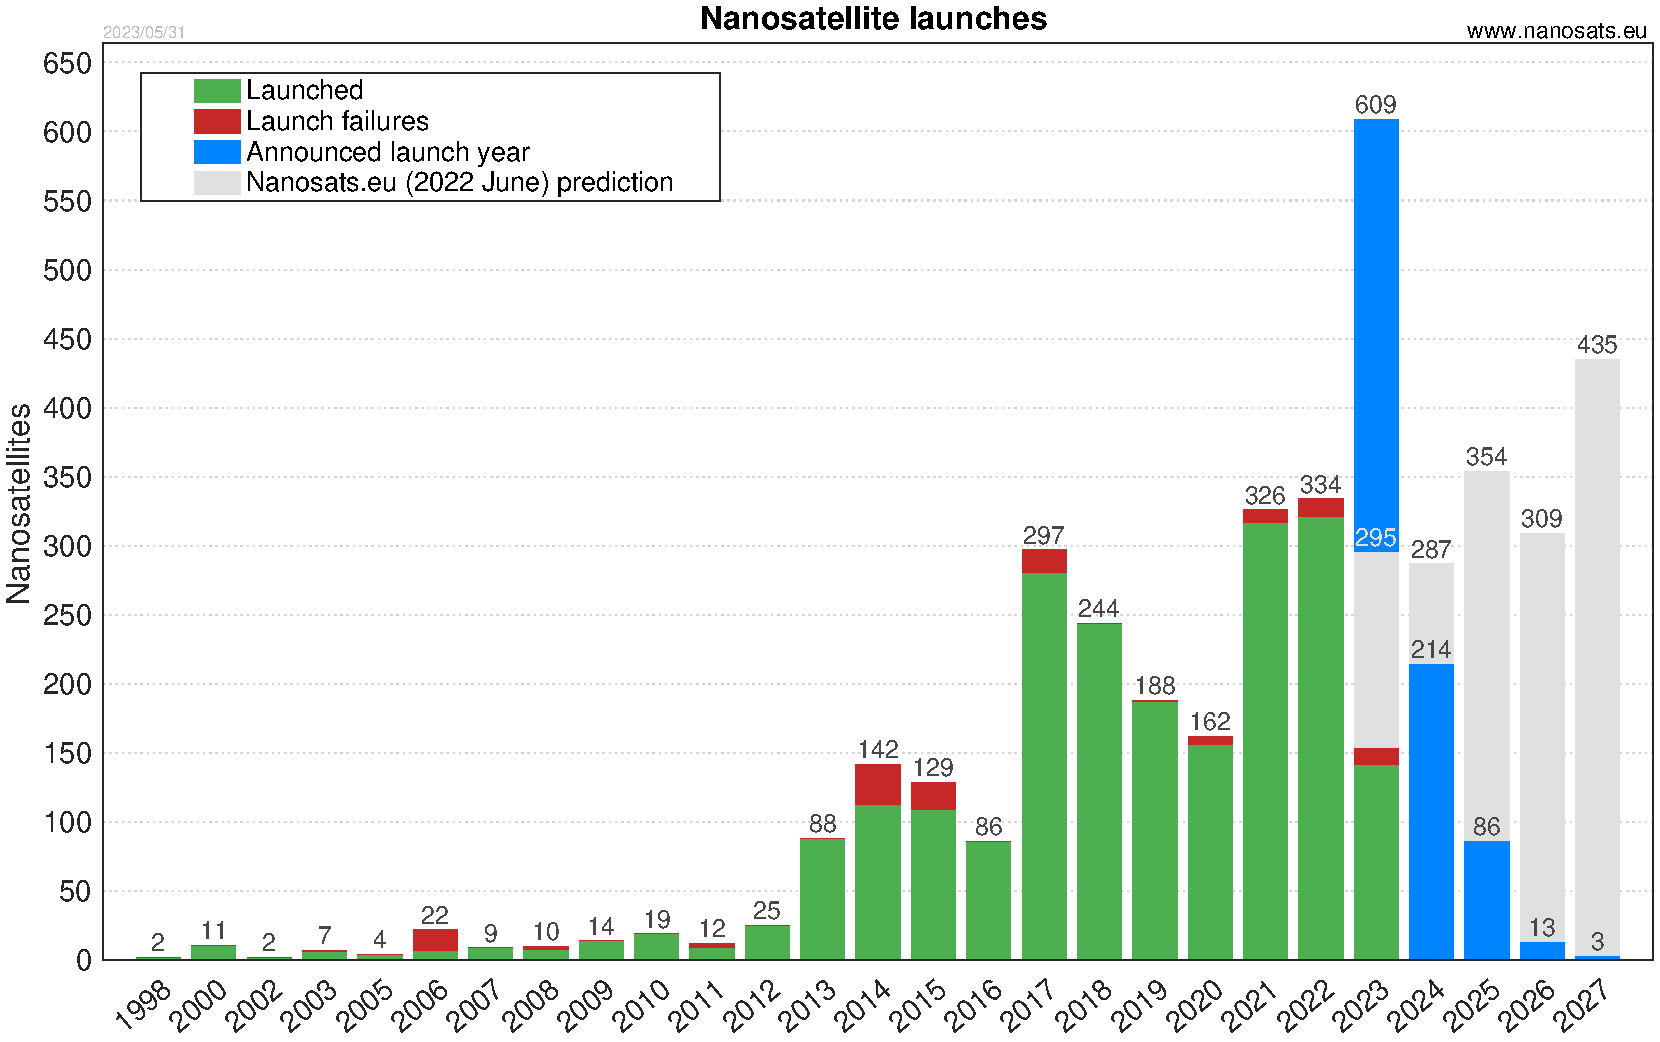
\includegraphics[width=\columnwidth]{figures/Nanosats_years_2023-05-31}
        \caption{Nanosatellite launches (2023/05/31) \cite{nanosatseu}.}
        \label{fig:cubesat-launches}
    \end{center}
\end{figure}

With a considerably lower cost, mainly due to the use of lower orbits such as LEO\nomenclature{\textbf{LEO}}{Low Earth Orbit.} (Low Earth Orbit) and COTS (Commercial Off-The-Shelf) components, it is becoming easier to develop and put this type of satellite into operation in space.

A standard that has dominated the nanosatellite market is the CubeSat standard \cite{cds}, which standardizes various physical characteristics for these types of satellites. This standard not only standardizes the space subsystems available on the market but also standardizes the launchers, which reduces the cost of launching a nanosatellite, which is one of the biggest costs within this type of project.

\section{Constellations}

Along with the rise of CubeSats, constellations of small satellites have emerged and grown in recent years. The low cost of this type of satellite, along with a significant recent increase in the number of launches, has also made it easier to create and deploy constellations of small satellites in low Earth orbit. With dozens or even hundreds of satellites in orbit, it is possible to achieve nearly constant coverage over the entire world. The chart in \autoref{fig:constellations} shows the status of the main nanosatellite constellations that are already in operation or planned for deployment.

\begin{figure}[!ht]
    \begin{center}
        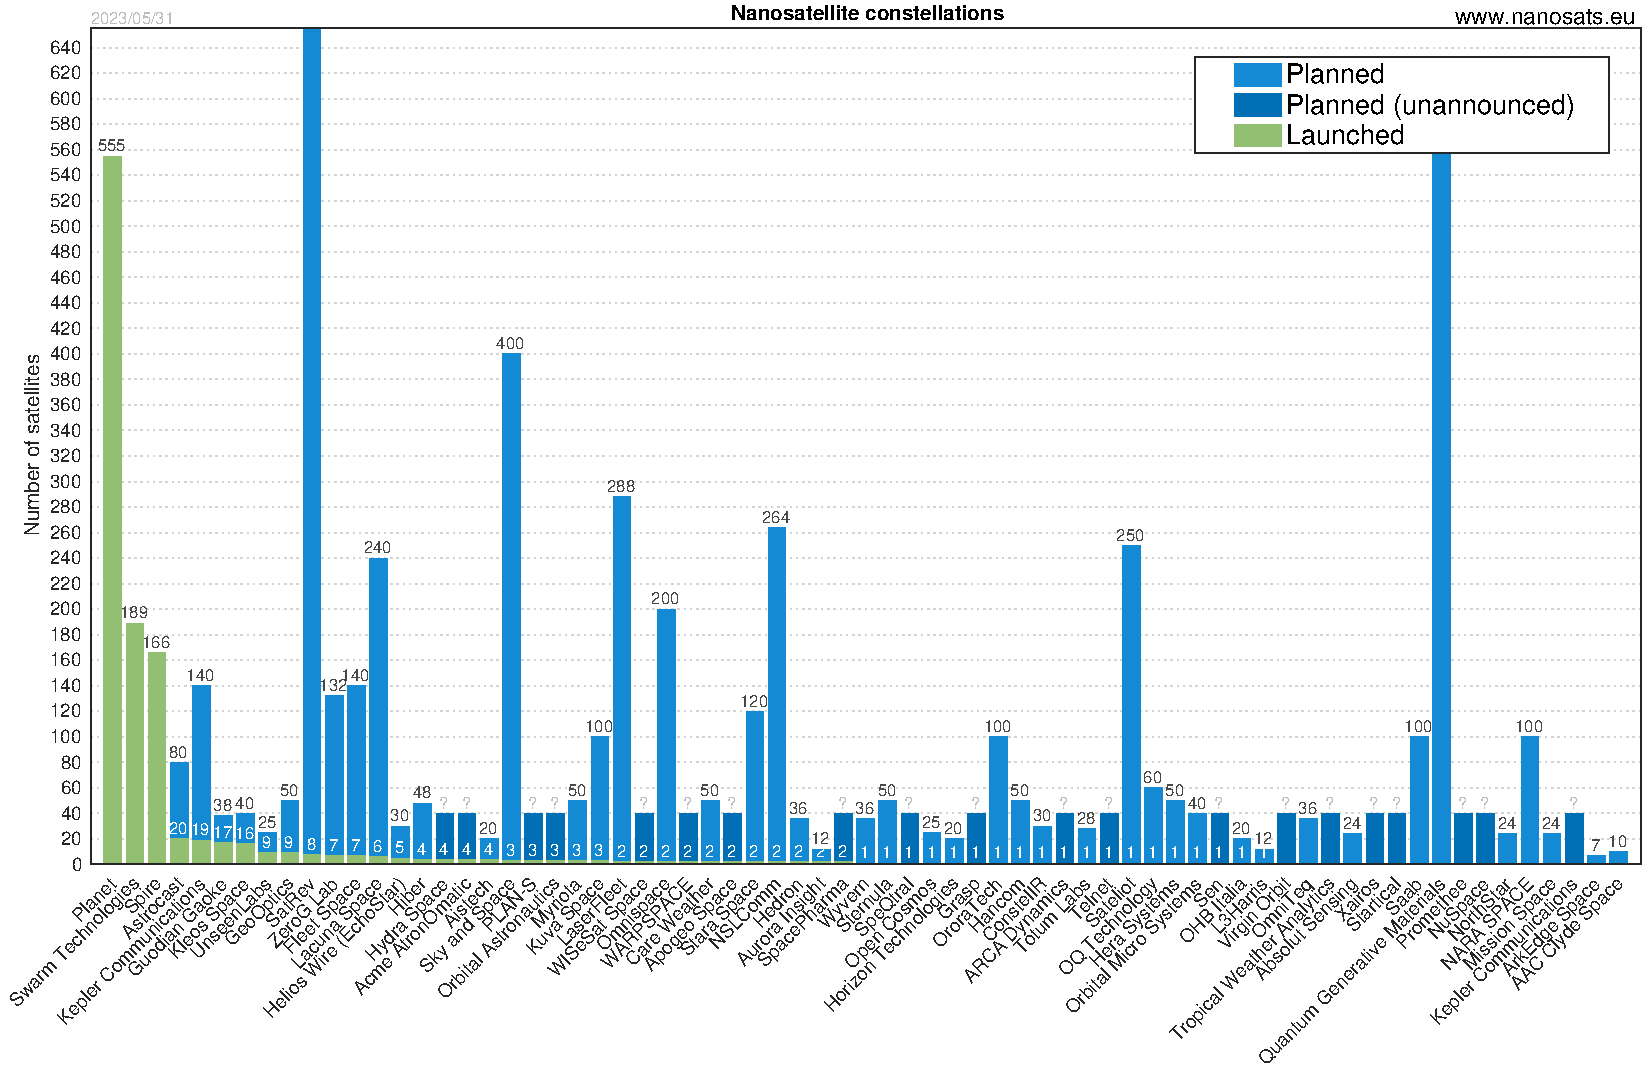
\includegraphics[width=\columnwidth]{figures/Nanosats_constellations_2023-05-31}
        \caption{Nanosatellite constellations (2023/05/31) \cite{nanosatseu}.}
        \label{fig:constellations}
    \end{center}
\end{figure}

\section{Motivation}

%Considerando o contexto apresentado acima a respeito do crescimento atual da utilização de pequenos satélites e da implatação de constelações dos mesmos, e ainda o rápido crescimento de dispositivos com necessidade de conexão a internet, denominadados Internet das Coisas (ou \textit{Internet of Things}, IoT), e outras tipos de tecnologias em ascenção como veículos autônomos, uma possível utilização dos nanossatélites seria em sistemas de navegação e localização, seja de cobertura específica para uma área, ou com cobertura global (GNSS).

%Considerando o contexto apresentado acima a respeito do crescimento atual da utilização de pequenos satélites e da implatação de constelações dos mesmos, uma possível utilização dos nanossatélites seria em sistemas de navegação e localização, seja de cobertura específica para uma área, ou com cobertura global (GNSS). O rápido crescimento de dispositivos com necessidade de conexão a internet, denominadados Internet das Coisas (ou \textit{Internet of Things}, IoT), e outras tipos de tecnologias em ascenção como veículos autônomos, tornam ainda mais atraente o uso desses tipos de satélites para aplicações desse tipo.

%Atualmente, os sistemas de navegação por satélite são compostos por satélites de grande porte operando em altitudes elevadas, normalmente em órbitas médias (MEO) ou até em órbitas geoestacionárias. Como será apresentado neste trabalho, a utilização de satélites de pequeno porte neste tipo de aplicação pode trazer algumas vantagens como um menor custo de implantação e operação, uma maior cobertura territorial e maior precisão, e até mesmos a simplificação de receptores em terra.

Considering the context presented above regarding the current growth of the use of small satellites and the implementation of constellations of these, a possible use of nanosatellites would be in navigation and location systems, either with specific coverage for an area or with global coverage (GNSS). The rapid growth of devices that require internet connection, known as the Internet of Things (IoT), and other emerging technologies such as autonomous vehicles, make the use of these types of satellites even more attractive for applications of this kind.

Currently, satellite navigation systems are composed of large satellites operating at high altitudes, typically in Medium Earth Orbits (MEO) or even in geostationary orbits (GEO). As will be presented in this work, the use of small satellites in this type of application can bring some advantages such as lower deployment and operation costs, greater territorial coverage and precision, and even the simplification of ground receivers.

\section{Objectives}

%Este trabalho tem como principal objetivo avaliar a possibilidade e viabilidade da implantação de um sistema de geolocalização baseado em satélites de pequeno porte, operando principalmente na forma de uma constelação em órbita baixa. O trabalho apresenta um estudo de órbita (como por exemplo o número de satélites necessários para um sistema desse tipo visando uma cobertura global), tecnologias disponíveis para a referência de tempo do sistema e outros subsistemas do satélite (neste caso especificamente para satélite de pequeno porte).

%Também tem-se como objetivo, o desenvolvimento de uma carga útil para a geração e transmissão de sinais de GNSS, a ser utilizada em um satélite de pequeno porte em uma missão projetada especificamente para testar e verificar o desempenho do sistema proposto.

The main objective of this work is to evaluate the possibility and feasibility of deploying a geolocation system based on small satellites, mainly operating in the form of a low Earth orbit constellation. The work presents an orbit study (such as the number of satellites required for such a system aiming at global coverage), technologies available for system time reference and other satellite subsystems (in this case, specifically for small satellites).

Another objective is to develop a payload for generating and transmitting GNSS signals, to be used on a small satellite in a mission designed specifically to test and verify the performance of the proposed system.

\section{Original contribution}

%Este trabalho tem como principal contribuição avaliar a viabilidade da implantação de um sistema de geolocalização baseado em pequenos satélites, explorando a possíveis tecnologias que podem ser utilizadas para a simplificação e/ou miniaturização dos componentes envolvidos do segmento espacial de um sistema deste tipo, um estudo de possíveis órbitas e tamanhos de constelação, e os requisitos necessários para os satélites do sistema.

%Como será demonstrado, há poucos trabalhos ou pesquisas acadêmicas semelhantes a este publicados até então. Já existem empresas explorando a possibilidade do uso de pequenos satélites em órbita baixa para o emprego de redes privadas de GNSS, mas nenhuma rede deste tipo já encontra-se em operação, todas encontram-se atualmente em fase de estudo e desenvolvimento. Portanto este trabalho pode ser considerado inovador e apresenta novos dados e informações para o área.

This work's main contribution is to evaluate the feasibility of implementing a geolocation system based on small satellites, exploring possible technologies that can be used to simplify and/or miniaturize the components involved in the space segment of such a system, a study of possible orbits and constellation sizes, and the necessary requirements for the system's satellites.

As will be demonstrated, there are few similar academic works or research published to date. There are already companies exploring the possibility of using small satellites in low orbit for the deployment of private GNSS networks, but no network of this type is currently in operation, all are still in the study and development phase. Therefore, this work can be considered innovative and presents new data and information for the field.

\section{Work organization}

%O \autoref{ch:related-work} apresenta uma revisão do estado da arte, comentando sobre o funcionamento de cada uma das redes atuais de GNSS, e apresentando os principais trabalhos relacionados, tanto a respeito da utilização de pequenos satéltes para este tipo de aplicação, quanto a repeito de tecnologias específicas que poderiam ser utilizadas para uma rede deste tipo.

%O \autoref{ch:problem-discussion} discute os principais problemas e questões a respeito da utilização de pequenos satélites e constelações dos mesmos para solucionar este tipo de problema. Neste capítulo apresenta-se possíveis tecnologias que poderiam ser utilizadas, questões de desempenho, entre outros.

%Já o \autoref{ch:proposed-work}, apresenta de forma detalhada o trabalha proposto, discutindo-se as principais questões a serem levadas em consideração neste tipo de problema, possíveis soluções que podem ser exploradas e análises preliminares.

Chapter \ref{ch:related-work} presents a review of the state of the art, commenting on the functioning of each of the current GNSS networks, and presenting the main related works, both regarding the use of small satellites for this type of application and regarding specific technologies that could be used for a network of this type.

Chapter \ref{ch:problem-discussion} discusses the main problems and issues regarding the use of small satellites and constellations of them to solve this type of problem. This chapter presents possible technologies that could be used, performance issues, among others.

Finally, \autoref{ch:proposed-work} presents in detail the proposed work, discussing the main issues to be taken into consideration in this type of problem, possible solutions that can be explored, and preliminary analyses.



% ChatPDF
%This document is a feasibility study of using small satellites for positioning networks, which aims to reduce costs and simplify deployment. The development of a payload containing a GNSS signal transmitter is also proposed to validate the concept. The document presents a review of the state of the art, commenting on the functioning of each of the current GNSS networks, and presenting the main related works, both regarding the use of small satellites for this type of application and regarding specific technologies that could be used for a network of this type. The implementation of the proposed system appears to be feasible based on the analysis carried out so far. The document also includes 3D representations and groundtracks obtained from simulations. Overall, this work can be considered innovative and presents new data and information for the field.